\chapter{Insights gained from individual CLIP-seq experiments}

\section{ABSTRACT}
Analysis of a single RBP, or comparison of binding patterns for mutant and wildtype RBPs can lead to novel biological insights.  In this chapter I present two short vignettes, both part of larger stories published elsewhere that illustrate the information gained when computational analysis on individual RNA binding proteins is performed.  In this chapter I briefly frame the biological question we sought to answer when analyzing two RBPs, UPF1 and MSI2, describe the computational analysis and summarize how these results contributed to the overall study.  
 
\section{INTRODUCTION}
ts\subsection{UPF1}
The dynamic interaction of RNA binding proteins (RBPs) with RNA is critical to every aspect of RNA metabolism\cite{Moore2005}. An important question yet to be fully addressed is how RNA regulators faithfully distinguish their target RNAs from the large complement of non-targets in the cell. Most models for RBP-target specificity invoke RBP affinity for target-specific RNA sequences, structures or bound proteins\cite{Anko2012, Glisovic2008}. However, for RNA quality control pathways, which detect and destroy faulty or non-functional RNAs, target-specific mechanisms for RBP recruitment are harder to envision, as these aberrant RNAs have the potential to differ widely in sequence composition and associated proteins\cite{VanHoof2011,Porrua2013}.

The first mRNA quality control pathway discovered was nonsense-mediated decay (NMD)\cite{Leeds1991, Losson1979, Maquat1981, Pulak1993}. This translation-dependent pathway is conserved among eukaryotes and degrades transcripts on which translation is halted by termination codons recognized as premature. In this way, NMD prevents accumulation of truncated polypeptides arising from aberrant mRNAs bearing premature termination codons (PTCs) and also serves as a potent gene suppression mechanism for select naturally occurring mRNAs, impacting the expression of up to 10\% of protein-coding genes in diverse eukaryotes\cite{Schweingruber2013}.

The key RNA binding regulator in NMD is Upf1, a helicase belonging to the SF1 family of DNA and RNA helicases\cite{Fairman-Williams2010}. Degradation of target mRNAs involves assembly of Upf1 with other NMD protein factors including Upf2 and Upf3 and, in most eukaryotes studied to date, the kinase Smg1 and one or more Smg5-7 proteins\cite{Kervestin2012, Schweingruber2013}. In humans, Smg1 phosphorylates Upf1 in a manner stimulated by Upf2, Upf3 and the exon junction complex\cite{Kashima2006}, which promotes association of phospho-binding proteins Smg5, Smg7 and mRNA decapping and deadenylation machinery\cite{Chakrabarti2014, Cho2013, Loh2013, Okada-Katsuhata2012}. Smg6 is itself an endonuclease, which has both phospho-dependent and -independent interactions with Upf1 \cite{Chakrabarti2014, Eberle2009, Nicholson2014, Okada-Katsuhata2012}. In addition, the ATPase activity of Upf1 itself has been implicated in a late step of target mRNA degradation to remodel the mRNP for enhanced nuclease access\cite{Franks2010}.

Despite the wealth of information regarding the processes involved in NMD target degradation, a fundamental, and yet poorly understood, aspect of the NMD pathway is what enables the central NMD factor Upf1 to distinguish target mRNAs from non-targets in the first place. NMD targets that have been well-studied share in common the fact that translation termination occurs at an unusual position in the mRNA – distal to the poly(A) tail due to an extended 3’UTR or with an exon-exon junction located downstream of termination\cite{Schweingruber2013}. One model for NMD target recognition proposes that stalled or aberrant termination complexes recruit Upf1\cite{Kervestin2012, Schweingruber2013}. Indeed, ribosome toe-printing assays in S. cerevisiae extracts and rabbit reticulocyte lysates revealed that ribosome dissociation at an NMD-inducing PTC compared to a normal termination codon (NTC) is stalled aberrantly\cite{Amrani2004, Peixeiro2012} and interactions between Upf1 and the ribosome release factors, eRF1 and eRF3, have been found in both yeast and human cells\cite{Czaplinski1998, Ivanov2008, Kashima2006, Singh2008}. Though the determinants leading to aberrant termination at a PTC have yet to be fully elucidated, it has been suggested that the absence of proximal mRNP factors that promote normal termination, such as poly(A) binding protein, underlies the difference between NMD targets and non-targets\cite{Cosson2002, Ivanov2008, Kervestin2012, Uchida2002}.

Recent reports cloud the simple view that aberrantly stalled translation termination complexes account fully for Upf1 recruitment to mRNAs. For example, Upf1 was found to associate with both target and non-target mRNAs even in the absence of translation, and the manner and degree to which translation affects Upf1-mRNA accumulation appears to vary among different mRNAs \cite{Hogg2010, Kurosaki2013a, Kurosaki2014, Zund2013}. Additionally, genome-wide crosslinking-immunoprecipitation studies have revealed that translation inhibitors induce a shift in Upf1 distribution across mRNAs, from a 3’ untranslated region bias to increased association with protein-coding regions \cite{Gregersen2014, Hurt2013, Zund2013}, suggesting that translation influences where Upf1 associates along the length of an mRNA, in addition to how strongly it associates with NMD target and non-target mRNAs overall.

Thus, the mechanisms involved in Upf1 discrimination of NMD target from non-target mRNAs have remained unclear. Here we present evidence that Upf1 ATPase activity is required for NMD target selection. In the absence of Upf1 ATPase activity, Upf1-mRNA selectivity is disrupted and NMD complexes accumulate indiscriminately on target and non-target mRNAs.

\subsection{MSI2}
Umbilical cord blood (CB)-derived hematopoietic stem cells (HSCs) are essential in many life saving regenerative therapies, but their low number in CB units has significantly restricted their clinical use despite the advantages they provide during transplantation\cite{Miller2013}. Select small molecules that enhance hematopoietic stem and progenitor cell (HSPC) expansion in culture have been identified\cite{Boitano2010, Fares2014}, however, in many cases their mechanisms of action or the nature of the pathways they impinge on are poorly understood. A greater understanding of the molecular pathways that underpin the unique human HSC self-renewal program will facilitate the development of targeted strategies that expand these critical cell types for regenerative therapies. Whereas transcription factor networks have been shown to influence the self-renewal and lineage decisions of human HSCs\cite{Novershtern2011, Laurenti2013}, the post-transcriptional mechanisms guiding HSC fate have not been closely Users investigated.  By performing a global analysis of MSI2-RNA interactions, we determined that MSI2 directly attenuates aryl hydrocarbon receptor (AHR) signaling through post-transcriptional downregulation of canonical AHR pathway components in CB HSPCs. Our study provides new mechanistic insight into RBP-controlled RNA networks that underlie the self-renewal process and give evidence that manipulating such networks ex vivo can provide a novel means to enhance the regenerative potential of human HSCs.

 
\section{RESULTS}

\subsection{Upf1-mRNA selectivity is lost on a transcriptome-wide level in Upf1 ATP-binding and ATP-hydrolysis mutants}
To examine the contribution of Upf1 ATPase activity to mRNA selectivity among endogenous mRNAs, we next turned to a global approach. We employed RIP-seq (RNA immunoprecipitation followed by strand-specific high-throughput sequencing) with Flag-tagged Upf1 WT, DEAA and KA expressed at endogenous levels (Figure 1 and S1A) to query the enrichment in IPs over inputs for endogenous RNAs in comparison to a parental cell line expressing no exogenous Upf1 used as a negative control. RIP-seq libraries were sequenced to a mean depth of 23 million reads and approximately twenty thousand genes had $>$0.1 RPKM per library. Significantly, Upf1 WT, DEAA and KA RIPs were all enriched for transcripts annotated as protein-coding with a smaller fraction derived from pseudogenes, indicating that the ATPase mutations do not disrupt Upf1 transcript specificity for mRNAs as a class.

Using the background recovery of RNAs in the negative control IPs to establish a 5\% false-discovery rate (Figure S1B), a distinct population of 2,040 Upf1-associated RNAs was identified as enriched by at least 2-fold over input levels (Figure 1A, Upf1-enriched genes indicated in red; Figure 1D). Based on observations by others \cite{Hogg2010, Kurosaki2014, Zund2013}, these RNAs likely include a mix of NMD sensitive mRNAs and mRNAs that are less sensitive to NMD but limited in downstream steps of the NMD pathway. In striking contrast to WT Upf1, RIPs for Upf1 DEAA and KA did not show enrichment for any RNAs when subjected to the same FDR cutoff (Figure S1B), and, accordingly, the population of WT Upf1-enriched RNAs was not enriched in Upf1 DEAA and KA RIPs over a WT Upf1-non-enriched RNA population defined by 0.97- to 1.03-fold enrichment in WT Upf1 RIPs over inputs (Figures 1A-C, compare red and blue; Figure 1D). These global findings generalize our observations for individual mRNA reporters to the human transcriptome, supporting the conclusion that RNA selectivity is lost in Upf1 mutants deficient in ATP binding or hydrolysis, despite their preserved specificity in associating with mRNAs as an RNA class.

\begin{figure}[ht]
  \centering
  \includegraphics[width=0.5\textwidth]{chapter_4_figures/Figure_2}
  \caption[Figure 1. Selectivity in mRNA association is lost on a transcriptome-wide level in Upf1 ATP binding- and ATP hydrolysis-deficient mutants]{(A-C) Scatter plots of reads per kilobase transcript per million mapped reads (RPKM) from RNA-seq of input samples versus IPs for Flag-Upf1 WT (A), DEAA (B) and KA (C). Genes with IP/input ratios for WT Upf1 of greater than 2.05 (cut-off based on 5\% false discovery rate (FDR) established by comparison to negative control cells expressing Flag epitope only, Figure S2) are shown in red (Upf1-enriched), while genes with log2 (IP/input) between -0.5 and +0.5 are shown in blue (non-enriched). All remaining genes are shown in grey. (D) Cumulative fraction of Upf1-enriched and non-enriched genes with IP enrichment represented as log2 (IP RPKM/input lysate RPKM) for Flag-Upf1 WT, KA, and DEAA, along with Flag only. Difference between WT Upf1 (Upf1-enriched) curve compared to all other curves was statistically significant (p-value $<$0.05 for all comparisons, KS-test). \index{Figure_1}}
  \label{fig:Figure_1}
  \end{figure}

\begin{figure}[ht]
  \centering
  \includegraphics[width=0.5\textwidth]{chapter_4_figures/Figure_S2}
  \caption[Supplementary Figure 1. Supplemental data related to RIP-RNAseq]{(A) Western blot of Flag-Upf1 recovered in RNA-IPs used for the RNA seq in Figure 2 alongside a two-fold titration of Flag-Upf1 WT input lysate. (B) Plot showing derivation of empirical false discovery rate (FDR) based on IP/input ratios for FLAG only, with X-axis as FDR and Y-axis as the number of genes remaining at that FDR threshold for all experiments. Inset depicts region around 5\% FDR cut-off (0.05) used for designating genes identified in WT Upf1 RNA-IP as Upf1-enriched. \index{Figure_S1}}
  \label{fig:Figure_S1}
\end{figure}

\subsection{ATP binding- and ATPase-deficient Upf1 accumulate on mRNA 3’UTRs and are enriched near termination codons and 3’ ends}
Our observations suggest that Upf1 ATPase activity is required for preventing Upf1 from accumulating and promoting NMD complex formation on translated non-target mRNAs. Recent studies employing Upf1 UV cross-linking IPs followed by high throughput sequencing (CLIP-seq) have reported that while Upf1 cross-links can be found all along the length of mRNAs, the overall distribution of binding sites has a distinct 3’UTR bias \cite{Gregersen2014, Hurt2013, Zund2013}. To gain insight into how binding to mRNA of Upf1 disrupted in the ATPase cycle might differ from WT Upf1, we performed UV CLIP-seq on Flag-Upf1 WT, DEAA and KA expressed at near endogenous levels (Figures S2A, B, C).

Notably, the binding site distributions of Upf1 DEAA and KA were nearly identical to each other and exhibited preference for mRNAs as a transcript class, with a 3’UTR bias similar to WT Upf1 (Figures 2A, and S2D, E). However, Upf1 mutant binding was strikingly shifted in comparison to WT Upf1 towards greater binding in 3’UTRs on average (Figure 2A; compare read densities in 3’UTRs for DEAA, KA with WT) and across all genes, as seen by the increased fraction of 3’UTR derived reads per mRNA normalized to length in Upf1 DEAA and KA CLIPs compared to WT Upf1 CLIP (Figure 2B, left graph, see right-shifted curves for DEAA, KA compared to WT; p-value $<$ 0.05, KS test). Examination of read distributions for the WT Upf1-enriched and non-enriched RNA subpopulations identified by RIP-seq (Figure 2) revealed that a greater fraction of the Upf1 enriched mRNAs had a stronger 3’UTR bias in WT Upf1 distribution than the non-enriched mRNAs, while the two sets of mRNAs were indistinguishable in their enhanced 3’UTR distribution bias for both Upf1 mutants (Figure 2B, right graph, compare dashed and solid lines). These findings suggest that Upf1 ATPase activity is needed to limit Upf1 association preferentially with 3’UTRs, and particularly so for the mRNA subpopulation that is less highly bound by WT Upf1 at steady state.

A closer examination of CLIP-seq read density at nucleotide resolution around translation termination codons and at mRNA 3’ ends revealed two peaks that are stronger for Upf1 DEAA and KA than WT Upf1. The first centers around 45 nucleotides downstream of the termination codon (Figure 2C, left), while the second peak was observed upstream of transcript 3’ ends (Figure 2C, right). This difference in binding site distribution between Upf1 mutants and WT Upf1 in regions proximal to the termination codon and the poly(A) tail was observed of both the WT Upf1-enriched and non-enriched mRNAs (Figure S2F). These observations suggest that the Upf1 ATPase cycle plays a particularly critical role in limiting accumulation of Upf1 at these specific sites in the 3’UTR.

\begin{figure}[ht]
  \centering
  \includegraphics[width=0.5\textwidth]{chapter_4_figures/Figure_6}
  \caption[Figure 2. Upf1 WT and ATPase mutants cross-link preferentially in 3’UTRs, with elevated crosslinking for ATPase mutants downstream of termination codons and near 3’ ends]{(A) Mean read density across the metagene, normalized to the total number of reads per gene. (B) Cumulative fraction of genes with 3’UTR read abundance represented as a fraction of total reads in the gene, normalized to nucleotide length, shown for all mRNAs on the left, and for WT enriched and non-WT enriched mRNAs, as defined in Figure 2, on the right. Differences between WT and mutant curves were statistically significant (p-value $<$ 0.001; KS statistic 0.30 for both DEAA and KA compared to WT for non-WT Enriched and 0.20 and 0.19 for DEAA and KA, respectively, compared to WT for WT Enriched) (C) Mean read densities, shown as percentages of total reads mapped in the region depicted per mRNA, around the first nucleotide of the translational stop codon, shown on the left, and the 3’ end of annotated transcripts, shown on the right. Solid lines represent regions where differences were found to be significant with a P-value $<$0.05 (Bonferroni corrected).
    \index{Figure_2}}
  \label{fig:Figure_2}
\end{figure}

\begin{figure}[ht]
  \centering
  \includegraphics[width=0.5\textwidth]{chapter_4_figures/Figure_S6}
  \caption[Supplementary Figure 2. Supplemental data related to CLIP-seq]{(A) Overview of workflow for CLIP-seq performed with Flag-Upf1 WT, DEAA and KA using $\alpha$-Flag antibodies for immunoprecipitation. (B) Anti-Flag Western blots of Flag-protein purification for CLIP-seq. (C) Film exposure of polyacrylamide resolved, 32P-end-labeled RNA that remained associated with Flag-Upf1 WT, DEAA and KA compared to Flag epitope-only, after 0.02U or 10U MNase digestion. The prominent band made apparent with 10U MNase treatment only in Flag-Upf samples migrates at a size consistent with Flag-Upf1. White box delineates region excised for CLIP-seq library construction. (D) Mean read density across the metagene, shown as a percentage of total reads in CLIPs for WT enriched and non-WT enriched genes, as defined in Figure 2, not normalized to the total number of reads per gene. (E) Cumulative fraction of genes with regional read abundance represented as a fraction of total reads in the gene, normalized to nucleotide length. UTR, untranslated region; CDS, coding sequence (F) Read density around stop codons and mRNA 3’ ends for WT-enriched and non-WT enriched genes. Solid and long-dash lines represent regions where differences were found to be significant with a P-value $<$0.05 (Bonferroni corrected). \index{Figure_S2}}
  \label{fig:Figure_S2}
\end{figure}


\subsection{MSI2 Global Analysis}

To identify key RNA targets that underlie MSI2 function, we analysed global MSI2 protein–RNA interactions using cross-linking immunoprecipitation followed by sequencing (CLIP–seq)\cite{Yeo2009} (Figure S3a, b). Replicates were highly correlated via gene RPKMs (reads per kilobase of transcript per million mapped reads) and 5,552 protein-coding genes were bound in both replicates (Figure S3c and Figure 3a, b). Within the top 40\% of reproducible clusters, MSI2 bound predominantly to the 3′ untranslated regions (3′UTRs) of mature mRNAs (Figure 3c). Importantly, 9\% of annotated protein-coding gene mRNAs were reproducible MSI2 targets, compared to 0.2\% of long non-coding RNAs (Figure S3d), suggesting that MSI2 controls the stability or translation of coding mRNAs. Motif analysis identified a consensus pentamer (U/G)UAGU resembling the known mouse Msi1-binding sequence\cite{Ohyama2012, Katz2014} within binding sites in all genic regions; additionally, MSI2-binding sites were generally significantly more conserved than background and tended to occur after the stop codon (Figure 3d and Figure S3e–h). The presence of MSI2 binding sites within Msi1 targets\cite{Katz2014} across species indicates that Musashi proteins may bind the same genes through 3′UTR-embedded motifs (Figure S3i). Finally, target gene ontology analysis revealed 186 biological processes categories, among the most significant of which were electron transport, oestrogen receptor signalling regulation and metabolism of small molecules, all processes known to be transcriptionally influenced by AHR signalling\cite{Tijet2005}.

Among the top 2\% of enriched CLIP–seq targets were the 3′UTRs of the genes for two AHR pathway components: heat shock protein 90 (HSP90) and CYP1B1. Each exhibited multiple MSI2-binding motifs correlating with overlapping clusters of CLIP–seq reads (Figure 3e and Figure S4a). To investigate the ability of MSI2 to post-transcriptionally regulate these genes during HSPC expansion, we looked for instances of uncoupled transcript and protein expression. HSP90 displayed uncoupling of transcript (1.6-fold up) and protein (1.6-fold down) expression early in culture, but after 7 days showed further upregulated transcript expression (2.5-fold) and variable protein levels (Figure 3f and Figure S4b). As AHR–HSP90 binding is essential for ligand-dependent transcriptional activity\cite{Mimura2003}, downregulation of HSP90 protein at the outset of HSPC culture would be expected to reduce latent AHR complex formation and attenuate AHR signalling. Indeed, CYP1B1 transcript and protein expression displayed twofold reductions early in culture, consistent with decreased AHR pathway activity; however, at day 7, CYP1B1 transcripts were upregulated 1.7-fold and uncoupled from protein expression, which was downregulated twofold (Figure 3g and Figure S4c). To test whether MSI2 directly mediates post-transcriptional repression of these targets, the 3′UTRs of CYP1B1 and HSP90 were coupled to luciferase. MSI2 overexpression induced significant reductions in luciferase signal from both reporters, and this effect was mitigated when the core CLIP–seq-identified UAG motifs were mutated (Figure S4d, e). As MSI2 overexpression-mediated post-transcriptional downregulation of the AHR pathway converged on CYP1B1 protein repression throughout culture, we explored the effects on HSPCs of inhibiting CYP1B1 independently with (E)-2,3`,4,5`-tetramethoxystilbene (TMS). During culture, TMS increased the frequency and total numbers of CD34+ cells by 1.5-fold and 2-fold, respectively (Figure 3h, i), phenocopying the effects of MSI2 overexpression. Finally, overexpression of both CYP1B1 lacking its 3′UTR and MSI2 decreased secondary CFU-GEMM replating efficiency (Figure S4f, g); this suggests that CYP1B1, while typically used to report AHR signalling, itself promotes HSPC differentiation.


\begin{figure}[ht]
  \centering
  \includegraphics[width=0.5\textwidth]{chapter_4_figures/Figure4_MSI}
  \caption[Figure 3. MSI2 overexpression post-transcriptionally downregulates AHR pathway components]{a, Overlap between MSI2 target genes from separate CLIP–seq experiments. b, Statistically significant overlap (P $<$ 0.0001, hypergeometric test) of clusters between the replicates. c, Percentage of CLIP–seq clusters in different genic regions. d, Consensus motifs within MSI2 clusters in different genic regions. P values presented for the top 40\% of clusters. e, CLIP–seq reads (blue, replicate 1; green, replicate 2) and clusters (purple) mapped to the 3′UTR of CYP1B1. Matches to the GUAG motif are shown in black. f, g, Immunofluorescence for HSP90 and CYP1B1 3 days after transduction and summary of fold-changes in HSP90 and CYP1B1 protein and transcript levels with MSI2 overexpression at 3 and 7 days after transduction (scale bar, 20 μm; dotted line indicates no change; n = 3 experiments). h, HSPC marker expression by CD34+ cells treated with TMS for 10 days. i, Absolute CD34+ cell number with TMS (n = 4 experiments). Data are presented as mean $\pm$ s.e.m. Unpaired t-test, **P $<$ 0.01.\index{Figure_3}}
  \label{fig:Figure_3}
\end{figure}

\begin{figure}[ht]
  \centering
  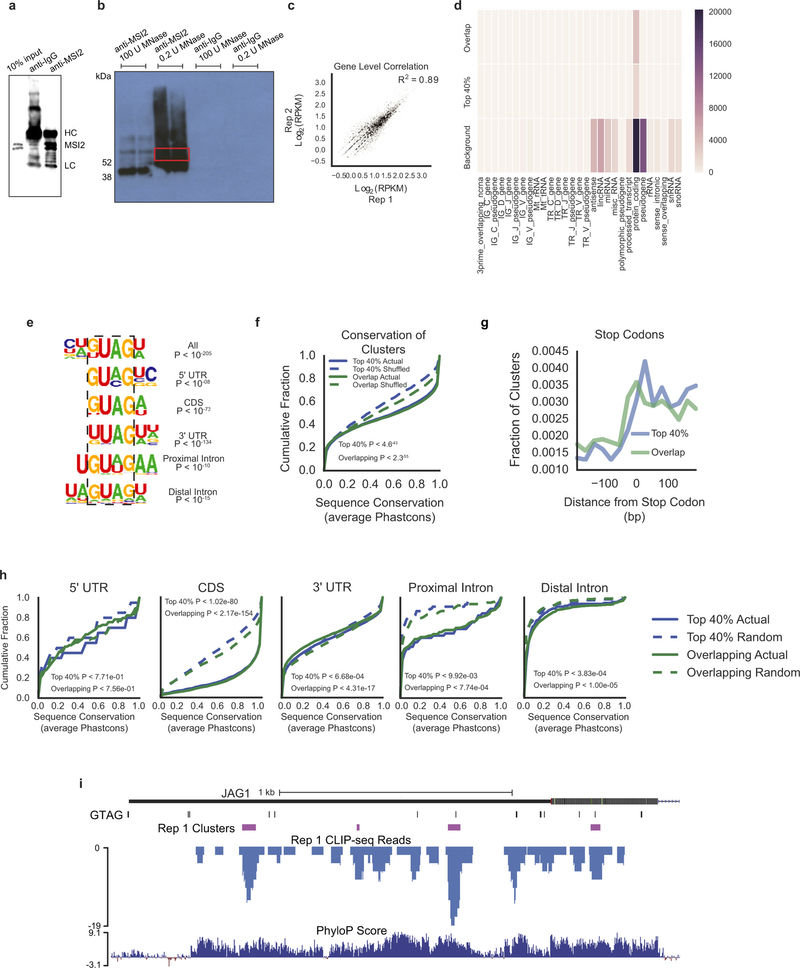
\includegraphics[width=0.5\textwidth]{chapter_4_figures/Figure_S9}
  \caption[Supplementary Figure 3. MSI2 preferentially binds mature mRNA within the 3'UTR]{a, Validation of the capacity of the anti-MSI2 antibody to immunoprecipitate MSI2 compared to IgG control pulldowns. b, Autoradiogram showing anti-MSI2 immunoprecipitated, MNase digested and radiolabelled RNA isolated for CLIP library construction and sequencing (red box). Low levels of MNase show a smearing pattern extending upwards from the modal weight of MSI2. c, Scatter plot of total number of uniquely mapped CLIP-seq reads for each gene, comparing both replicates. d, Heatmap indicating the number of different classes of Gencode annotated genes that contain at least one predicted MSI2 binding site. e, Consensus motifs within MSI2 clusters in the different genic regions. P-values for the most statistically significant enriched motif is presented for all overlapping clusters between replicates. f, Cumulative distribution function of mean conservation score (Phastcons) of MSI2 clusters, compared to a shuffled background control, computed for all overlapping clusters and the top 40\% of overlapping clusters. P- values were obtained by a Kolgomorov-Smirnov two-tailed test comparing the distributions from actual and shuffled locations. g, Number of clusters within 200 bases of the annotated stop codon in known mRNA transcripts for all overlapping clusters between replicates and the top 40\% of overlapping clusters. h, Cumulative distribution function of mean conservation score (Phastcons) of MSI2 clusters, compared to a shuffled background control, computed for overlapping clusters between the replicates and the top 40\% of overlapping clusters found in different genic regions. Similarity in the 3'UTR conservation for the top 40\% with the shuffled background control is likely due to MSI2 sites being small and not needing structural contexts for conservation. P-values were obtained by a Kolgomorov-Smirnov two-tailed test comparing the distributions from actual and shuffled locations. i, Genome browser views displaying CLIP-seq mapped reads from replicate 1 (blue), predicted clusters (purple), exact matches for the GUAG sequence (black) and mammal conservation scores (PhyloP) in the 3' UTRs for a previously predicted Msi1 target. \index{Figure_S3}}
  \label{fig:Figure_S3}
\end{figure}

\begin{figure}[ht]
  \centering
  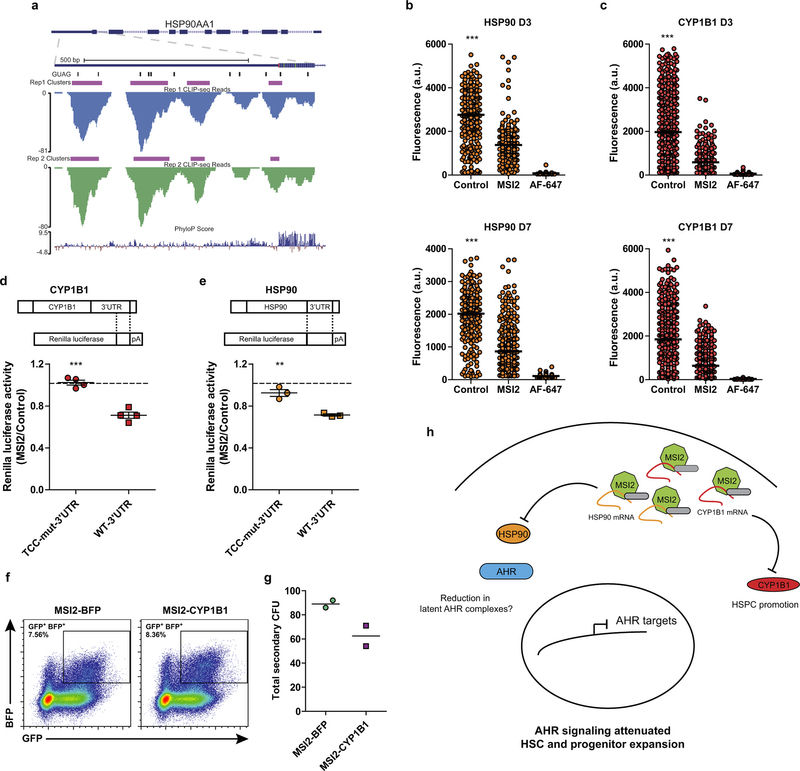
\includegraphics[width=0.5\textwidth]{chapter_4_figures/Figure_S10}
  \caption[Supplementary Figure 4. MSI2 OE represses CYP1B1 and HSP90 3'UTR Renilla Luciferase reporter activity]{a, CLIP-seq reads (replicate 1 in blue and replicate 2 in green) and clusters (purple) mapped to the 3'UTR of HSP90. Matches to the GUAG motif are shown in black. Mammal PhyloP score listed in last track. b and c, Representative data of mean per cell fluoresence for HSP90 and CYP1B1 protein in transduced CD34+ CB. Protein level in cells during in vitro culture was analyzed 3 days (D3) and 7 days (D7) after transduction and sorting for GFP. Corresponding secondary alone antibody staining is shown for each experiment. Each circle represents a cell, and greater than 200 cells were analyzed per condition. d and e, Levels of renilla luciferase activity in NIH-3T3 cells co-transfected with control or MSI2 OE vectors and the CYP1B1 or HSP90 wild type or TCC mutant 3'UTR luciferase reporter (dotted line indicates no change in renilla activity; n=4 CYP1B1 and n=3 HSP90 experiments). f, Flow plots of co-transduced CD34+ CB cells with MSI2 (GFP) and CYP1B1 (BFP) lentivirus. g, GFP+ BFP+ CFU-GEMMs generated from f were replated in to secondary CFU assays and enumerated for total number of colonies formed. A total of 24 CFU-GEMMs from MSI2- BFP and MSI2-CYP1B1 were replated (n=2 experiments). Data presented as mean ± SEM. ***p$<$0.001, **p$<$0.01. h, A model for AHR pathway attenuation through MSI2 post- transcriptional processing. MSI2 mediates the post-transcriptional down regulation of HSP90 at the outset of culture and continuously represses the prominent AHR pathway effector CYP1B1 to facilitate HSPC expansion. The resultant MSI2-mediated repression of AHR signaling enforces a self-renewal program and allows HSPC expansion ex vivo. \index{Figure_S4}}
  \label{fig:Figure_S4}
\end{figure}

\section{METHODS}

\subsection{RIP sample preparation for Western, Northern or RNA-seq analysis}
To monitor protein depletions, if used, and recovery of Flag- or Myc-epitope tagged proteins and/or coprecipitating proteins, a fraction of the input lysate and IP was set aside for Western blotting in 1x SDS loading buffer (60 mM Tris-HCl, pH 6.8, 2\% SDS, 4\% β-mercaptoethanol, 10\% glycerol, 0.1\% bromophenol blue and xylene cyanol). To monitor RNA, Trizol (Ambion) was added to input, unbound, and IP samples. RNA was isolated according to the manufacturer, with 25 μg linear polyacrylamide used as carrier for either library preparation for RNA-seq analysis (see below) or Northern blotting. 

\subsection{RIP-seq and CLIP-seq analysis}
Sequence alignment of CLIP-seq and RIP-seq data to the human genome.
Sequencing reads from CLIP-seq and RIP-seq libraries were first trimmed of polyA tails, adapters, and low quality ends using cutadapt with parameters --match-read-wildcards --times 2 -e 0 -O 5 --quality-cutoff' 6 -m 18 -b TCGTATGCCGTCTTCTGCTTG -b ATCTCGTATGCCGTCTTCTGCTTG -b CGACAGGTTCAGAGTTCTACAGTCCGACGATC -b TGGAATTCTCGGGTGCCAAGG -b AAAAAAAAAAAAAAAAAAAAAAAAAAAAAAAAAAAAAAAAAAAAAAAAAA -b TTTTTTTTTTTTTTTTTTTTTTTTTTTTTTTTTTTTTTTTTTTTTTTTTT. Reads were then mapped against a database of repetitive elements derived from RepBase18.05. Bowtie version 1.0.0 with parameters -S -q -p 16 -e 100 -l 20 was used to align reads against an index generated from Repbase sequences \cite{Langmead2009}. Reads not mapped to Repbase sequences were aligned to the hg19 human genome (UCSC assembly) using STAR \cite{Dobin2013a} version 2.3.0e with parameters --outSAMunmapped Within –outFilterMultimapNmax 1 –outFilterMultimapScoreRange 1.


\subsection{CLIP-seq Cluster Identification and analyses.}
Reads that were PCR replicates were removed from each CLIP-seq library using a custom script. Briefly one read was kept at each nucleotide position when more than one read’s 5' end was mapped. Clusters were then assigned using the CLIPper software with parameters --bonferroni --superlocal --threshold- software \cite{Lovci2013}. Clusters that overlap by at least one base pair are considered overlapping clusters, as determined using bedtools \cite{Quinlan2010} and pybedtools\cite{Dale2011a}.

\subsection{Read Distribution Region Counting and comparisons.}
Genic features were defined using gencode v17 annotations \cite{Harrow2006}. For each gene, all annotated transcripts for that gene were combined and gene level features were generated. 5' UTR, CDS, and 3' UTR regions from gencode genes were identified and merged at the gene level. The number of reads mapping to each annotated meta-region for each gene was counted. Each gene region (3' and 5' UTRs and CDS) was binned into 100 bins, and the mean of reads in each bin was calculated. Then for all genes, the mean of each bin was calculated and plotted. Finally, for each experiment the distribution was normalized to compute a probability density across each bin. To compare different regions, the total number of reads within each region was totaled. For each region the RPK (reads per 1,000 bases) was calculated. To find the percent of reads falling into each region, the percent of RPK normalized reads that were contained within a given region per gene was calculated.

\subsection{Read Distribution Feature Counting.}
For read distributions around specific genic features (termination codons and 3’ transcript ends), features from gencode v17 were selected, the number of reads around each feature was counted, and the mean for each base was calculated across all features. Finally, for each experiment the distribution was normalized to show a probability density across each bin. A background model was generated assuming a uniform distribution of reads distributed to each base, and reads were normally distributed. Each feature at each base is then an independent observation and a z-test was applied to each base (Bonferroni corrected) to see if the reads at that base differed significantly from the background distribution.

\subsection{RIP-seq Analysis.}
RPKMs for each gene annotated in gencode v17 were calculated from RIP-seq data using custom scripts. We determined the fold-change (log2) threshold by which at most 5\% of genes in the FLAG RIP-seq sample were “enriched”. This threshold reflected a false discovery rate (FDR) of 5\%, and was applied to both WT Upf1 and mutant Upf1 RIP-seq samples to identify Upf1 target genes. Non-targets were defined as having a log2 fold change in WT Upf1 RIPs of between -0.05 and 0.05 RPKM

\subsection{UV CLIP–seq library preparation}
CLIP–seq was performed as previously described\cite{Yeo2009}. Briefly, 25 million NB4 cells (a transformed human cell line of haematopoietic origin) were washed in PBS and UV-cross-linked at 400 mJ cm−2 on ice. Cells were pelleted, lysed in wash buffer (PBS, 0.1\% SDS, 0.5\% Na-deoxycholate, 0.5\% NP-40) and DNase-treated, and supernatants from lysates were collected for immunoprecipitation. MSI2 was immunoprecipitated overnight using 5 μg of anti-MSI2 antibody (EP1305Y, Abcam) and Protein A Dynabeads (Invitrogen). Beads containing immunoprecipated RNA were washed twice with wash buffer, high-salt wash buffer (5× PBS, 0.1\% SDS, 0.5\% Na-Deoxycholate, 0.5\% NP-40), and PNK buffer (50 mM Tris-Cl pH 7.4, 10 mM MgCl2, 0.5\% NP-40). Samples were then treated with 0.2 U MNase for 5 min at 37° with shaking to trim immunopreciptated RNA. MNase inactivation was then carried out with PNK + EGTA buffer (50 mM Tris-Cl pH 7.4, 20 mM EGTA, 0.5\% NP-40). The sample was dephosphorylated using alkaline phosphatase (CIP, NEB) at 37° for 10 min followed by washing with PNK+EGTA, PNK buffer, and then 0.1 mg ml−1 BSA in nuclease-free water. 3′RNA linker ligation was performed at 16° overnight with the following adaptor: 5′P-UGGAAUUCUCGGGUGCCAAGG-puromycin. Samples were then washed with PNK buffer, radiolabelled using P32-y-ATP (Perkin Elmer), run on a 4-12\% Bis-Tris gel and then transferred to a nitrocellulose membrane. The nitrocellulose membrane was developed via autoradiography and RNA–protein complexes 15–20 kDa above the molecular weight of MSI2 were extracted with proteinase K followed by RNA extraction with acid phenol-chloroform. A 5′RNA linker (5′HO-GUUCAGAGUUCUACAGUCCGACGAUC-OH) was ligated to the extracted RNA using T4 RNA ligase (Fermentas) for 2 h and the RNA was again purified using acid phenol-chloroform. Adaptor ligated RNA was re-suspended in nuclease-free water and reverse transcribed using Superscript III reverse transcriptase (Invitrogen). Twenty cycles of PCR were performed using NEB Phusion Polymerase using a 3′PCR primer that contained a unique Illumina barcode sequence. PCR products were run on an 8\% TBE gel. Products ranging between 150 and 200 bp were extracted using the QIAquick gel extraction kit (Qiagen) and re-suspended in nuclease-free water. Two separate libraries were prepared and sent for single-end 50-bp Illumina sequencing at the Institute for Genomic Medicine at the University of California, San Diego. 47,098,127 reads from the first library passed quality filtering, of which 73.83\% mapped uniquely to the human genome. 57,970,220 reads from the second library passed quality filtering, of which 69.53\% mapped uniquely to the human genome. CLIP-data reproducibility was verified through high correlation between gene RPKMs and statistically significant overlaps in the clusters and genes within replicates. CLIP–seq data have been deposited in NCBI’s GEO and are accessible through GEO Series accession number GSE69583.


\subsection{CLIP–seq mapping and cluster identification}
Before sequence alignment of CLIP–seq reads to the human genome was performed, sequencing reads from libraries were trimmed of polyA tails, adapters, and low quality ends using Cutadapt with parameters -match-read-wildcards -times 2 -e 0 -O 5 -quality-cutoff 6 -m 18 -b TCGTATGCCGTCTTCTGCTTG -b ATCTCGTATGCCGTCTTCTGCTTG -b CGACAGGTTCAGAGTTCTACAGTCCGACGATC -b TGGAATTCTCGGGTGCCAAGG -b AAAAAAAAAAAAAAAAAAAAAAAAAAAAAAAAAAAAAAAAAAAAAAAAAA -b TTTTTTTTTTTTTTTTTTTTTTTTTTTTTTTTTTTTTTTTTTTTTTTTTT. Reads were then mapped against a database of repetitive elements derived from RepBase (version 18.05). Bowtie (version 1.0.0) with parameters -S -q -p 16 -e 100 -l 20 was used to align reads against an index generated from Repbase sequences\cite{Langmead2009}. Reads not mapped to Repbase sequences were aligned to the hg19 human genome (UCSC assembly) using STAR (version 2.3.0e)\cite{Dobin2013a} with parameters -outSAMunmapped Within -outFilterMultimapNmax 1 -outFilterMultimapScoreRange 1. To identify clusters in the genome of significantly enriched CLIP-seq reads, reads that were PCR replicates were removed from each CLIP–seq library using a custom script of the same method as in \cite{Darnell2012}; otherwise, reads were kept at each nucleotide position when more than one read’s 5′-end was mapped. Clusters were then assigned using the CLIPper software with parameters -bonferroni -superlocal-threshold\cite{Lovci2013}. The ranked list of significant targets was calculated assuming a Poisson distribution, where the observed value is the number of reads in the cluster, and the background is the number of reads across the entire transcript and or across a window of 1000 bp $\pm$ the predicted cluster.

\subsection{Gene annotations for CLIP–seq}
Transcriptomic regions and gene classes were defined using annotations found in gencode v17. Depending on the analysis, clusters were associated by the Gencode-annotated 5′UTR, 3′UTR, CDS or intronic regions. If a cluster overlapped multiple regions, or a single part of a transcript was annotated as multiple regions, clusters were iteratively assigned first as CDS, then 3′UTR, 5′UTR and finally as proximal ($<$500 bases from an exon) or distal ($>$500 bases from an exon) introns. Overlapping peaks were calculated using bedtools and pybedtools\cite{Quinlan2010, Dale2011a}.

\subsection{Gene ontology analysis for CLIP–seq}
Significantly enriched gene ontology (GO) terms were identified using a hypergeometric test that compared the number of genes that were MSI2 targets in each GO term to genes expressed in each GO term as the proper background. Expressed genes were identified using the control samples in SRA study SRP012062. Mapping was performed identically to CLIP–seq mapping, without peak calling and changing the STAR parameter outFilterMultimapNmax to 10. Counts were calculated with featureCounts37 and RPKMs were then computed. Only genes with a mean RPKM $>$ 1 between the two samples were used in the background expressed set.

\subsection{De novo motif and conservation analysis for CLIP–seq}
Randomly located clusters within the same genic regions as predicted MSI2 clusters were used to calculate a background distribution for motif and conservation analyses. Motif analysis was performed using the HOMER algorithm as in \cite{Lovci2013}. For evolutionary sequence conservation analysis, the mean (mammalian) phastCons score for each cluster was used.
